\documentclass[runningheads]{llncs}
\usepackage{amsmath}
\usepackage{amsfonts}
\usepackage{mathtools}
\usepackage{color}
\usepackage{graphicx}
\usepackage{listings}
\usepackage{wasysym}
\usepackage[lighttt]{lmodern}
\usepackage{siunitx}
% If you use the hyperref package, please uncomment the following line
% to display URLs in blue roman font according to Springer's eBook style:
% \renewcommand\UrlFont{\color{blue}\rmfamily}

\newcommand\Dist{\mathit{Dist}}
\newcommand\ctrl{\mathit{ctrl}}
\newcommand\prnt{\mathit{prnt}}
\newcommand\link{\mathit{link}}
\newcommand\points{\mathit{points}}
\newcommand\ports{\mathit{ports}}
\newcommand\ar{\mathit{ar}}
\newcommand\id{\mathsf{id}}
\newcommand\Id{\mathsf{Id}}

\providecommand\longrightarrowRHD{\relbar\joinrel\relbar\joinrel\mathrel\RHD}
\providecommand\longrightarrowrhd{\relbar\joinrel\relbar\joinrel\mathrel\rhd}
\providecommand\longrightdoublearrowRHD{\mathrel\LHD\joinrel\relbar\joinrel\relbar\joinrel\mathrel\RHD}

\makeatletter
\providecommand*\xrightarrowRHD[2][]{\ext@arrow 0055{\arrowfill@\relbar\relbar\longrightarrowRHD}{#1}{#2}}
\providecommand*\xrightarrowrhd[2][]{\ext@arrow 0055{\arrowfill@\relbar\relbar\longrightarrowrhd}{#1}{#2}}
\makeatother

\lstdefinelanguage{Big}{
  basicstyle=\ttfamily,
  sensitive=true,
  morekeywords={fun, brs, end, sbrs, pbrs, nbrs, begin, init, atomic, preds,
    rules, action, big, ctrl, float, int, react},
  comment=[l]{\#}
}

\ttfamily
\DeclareFontShape{OT1}{lmtt}{m}{it}
     {<->sub*lmtt/m/sl}{}

\begin{document}
\title{Nondeterministic Bigraphical Reactive Systems for Markov Decision
  Processes\thanks{Supported by organization x.}}
\titlerunning{Nondeterministic BRSs for MDPs}
\author{Paulius Dilkas}
\authorrunning{P. Dilkas}
\institute{University of Glasgow, Glasgow, UK}
\maketitle

\begin{abstract}
The abstract should briefly summarize the contents of the paper in
150--250 words.

\keywords{Bigraphs \and Bigraphical Reactive Systems \and Probabilistic
  semantics \and Markov decision process.}
\end{abstract}

\section{Introduction}

\subsection{Markov Decision Processes}

\begin{definition}[Markov decision process] \label{mdp}
  For any finite set $X$, let $\Dist(X)$ denote the set of discrete probability
  distributions over $X$. A \emph{Markov Decision Process} is a tuple $ (S,
  \overline{s}, A, P, L)$, where: $S$ is a finite set of states and
  $\overline{s} \in S$ is the initial state; $A$ is a finite set of
  \emph{actions}; $P : S \times A \to \Dist(S)$ is a (partial) probabilistic
  transition function, mapping state-action pairs to probability distributions
  over $S$; $L : S \to 2^P$ is a labelling with atomic propositions.
\end{definition}

\begin{definition}[rewards]
  A \emph{reward structure} for an MDP $(S, \overline{s}, A, P, L)$ is a pair
  $(\rho, \iota)$, where $\rho : S \to \mathbb{R}$ is the \emph{state reward
    function}, and $\iota : S \times A \to \mathbb{R}$ is the \emph{transition
    reward function}.
\end{definition}

\subsection{Bigraphs}

% TODO: introduce bigrapher
From \cite{dblp:journals/tcs/sevegnanic15}.
From PhD thesis \cite{DBLP:phd/ethos/Sevegnani12}

\begin{figure}
  \centering
  \includegraphics{models/example_bigraph/foo_lhs.pdf}
  \caption{An example bigraph.}
  \label{example_bigraph}
\end{figure}

Consider the graphical representation of a bigraph in Fig.
\ref{example_bigraph}. The white ellipses are the \emph{nodes}. Each node has a
type, called \emph{control}, denoted here by the labels \textsf{A}, \textsf{B},
and \textsf{C}. The two white dashed rectangles represent \emph{regions},
i.e. parents of any otherwise parentless nodes. Grey dashed rectangles are
called \emph{sites} and encode parts of the model that have been abstracted
away. Nodes, sites, and regions are also known as \emph{places}. Two places with
the same parent, or two points with the same link are called \emph{siblings}.

\begin{definition}[concrete place graph with sharing]
  A \emph{concrete place graph with sharing}
  \[ F = (V_F, \ctrl_F, \prnt_F) : m \to n \]
  is a triple having an inner interface $m$ and an outer interface $n$. These
  index the sites and regions of the place graph, respectively. $F$ has a finite
  set $V_F \subset \mathcal{V}$ of nodes, a control map $\ctrl_F : V_F \to
  \mathcal{K}$, and a \emph{parent relation}
  \[ \prnt_F \subseteq (m \uplus V_F) \times (V_F \uplus n) \]
  that is acyclic, i.e., $(v, v) \not\in \prnt_F^+$ for any $v \in V_F$.
\end{definition}

\begin{definition}[composition for place graphs with sharing]
  If $F : k \to m$ and $G : m \to n$ are two concrete place graphs with sharing
  with $V_F \cap V_G = \emptyset$, their composite
  \[ G \circ F = (V, \ctrl, \prnt) : k \to n \]
  has nodes $V = V_F \uplus V_G$ and control map $\ctrl = \ctrl_F \uplus
  \ctrl_G$. Its parent relation $\prnt \subseteq (k \uplus V) \times (V \uplus
  n)$ is given by:
  \[ \prnt \coloneqq \prnt_G^\lhd \uplus \prnt_\circ \uplus \prnt_F^\rhd, \]
  where
  \begin{align*}
    \prnt_F^\rhd &= \prnt_F \rhd V_F, \\
    \prnt_G^\lhd &= V_G \lhd \prnt_G, \\
    \prnt_\circ &= (m \lhd \prnt_G) \circ (\prnt_F \rhd m).
  \end{align*}
\end{definition}

\begin{definition}[tensor product for place graphs]
  If $G_0 : m_0 \to n_0$ and $G_1 : m_1 \to n_1$ are two concrete place graphs
  with sharing with $V_F \cap V_G = \emptyset$, their tensor product
  \[ G_0 \otimes G_1 = (V, \ctrl, \prnt) : m_0 + m_1 \to n_0 + n_1 \]
  has nodes $V = V_{G_0} \uplus V_{G_1}$ and control map $\ctrl \coloneqq
  \ctrl_{G_0} \uplus \ctrl_{G_1}$. Its parent relation $\prnt \subseteq [(m_0 +
  m_1) \uplus V] \times [V \uplus (n_0 + n_1)]$ is defined as
  \[ \prnt_{G_0} \uplus \prnt_{G_1}^{(m_0, n_0)}, \]
  where
  \begin{align*}
    \prnt_{G_1}^{(m_0, n_0)} = &\{ (v, w) \mid (v, w) \in \prnt_{G_1} \text{ and } v, w \in V_{G_1} \} \\
    \uplus &\{ (m_0 + i, w) \mid (i, w) \in \prnt_{G_1}, w \in V_{G_1} \text{ and } i \in m_1 \} \\
    \uplus &\{ (v, n_0 + i) \mid (v, i) \in \prnt_{G_1}, v \in V_{G_1} \text{ and } i \in n_1 \} \\
    \uplus &\{ (m_0 + i, n_0 + j) \mid (i, j) \in \prnt_{G_1}, i \in m_1, \text{ and } j \in n_1 \}.
  \end{align*}
\end{definition}

\begin{definition}[concrete link graph]
  A \emph{concrete link graph}
  \[ F = (V_F, E_F, \ctrl_F, \link_F) : X \to Y \]
  is a quadruple having an inner face $X$ and an outer face $Y$, both finite
  subsets of $\mathcal{X}$, called respectivelly the inner and outer names of
  the link graph. $F$ has finite sets $V_F \subset \mathcal{V}$ of nodes and
  $E_F \subset \mathcal{E}$ of edges, a control map $\ctrl_F : V_F \to
  \mathcal{K}$ and a \emph{link map}
  \[ \link_F : X \uplus P_F \to E_F \uplus Y, \]
  where $P_F \coloneqq \{ (v, i) \mid i \in \ar(\ctrl_F(v)) \}$ is the set of
  ports of $F$. Thus $(v, i)$ is the $i$th port of node $v$. We shall call $X
  \uplus P_F$ the \emph{points} of $F$, and $E_F \uplus Y$ its \emph{links}.
\end{definition}

The sets of points and the set of ports of a link $l$ are defined by
\[ \points_F(l) \coloneqq \{ p \mid \link_F(p) = l \}, \quad \ports_F(l)
  \coloneqq \points_F(l) \setminus X. \]
An edge is \emph{idle} if it has no points. Identities over name sets are
defined by $\id_X = (\emptyset, \emptyset, \emptyset, \Id_X) : X \to X$.

\begin{definition}[concrete bigraph with sharing]
  A concrete bigraph
  \[ F = (V_F, E_F, \ctrl_F, \prnt_F, \link_F) : \langle k, X \rangle \to
    \langle m, Y \rangle \]
  consists of a concrete place graph with sharing $F^P = (V_F, \ctrl_F, \prnt_F)
  : k \to m$ and a concrete link graph $F^L = (V_F, E_F, \ctrl_F, \link_F) : X
  \to Y$. We write the concrete bigraph with sharing as $F = (F^P, F^L)$.
\end{definition}

Given a set of reaction rules, we refer to the configurations that a system may
adopt as \emph{states}. A bigraph with inner face $\epsilon$ is called
\emph{ground}.

\begin{definition}[solid bigraph]
  A bigraph is \emph{solid} if these conditions hold:
  \begin{enumerate}
  \item no regions or outer names are idle (a region is called \emph{idle}
    if it is empty);
  \item no two sites or inner names are siblings;
  \item the parent of every site is a node;
  \item no outer name is linked to an inner name.
  \end{enumerate}
\end{definition}

\begin{definition}[reaction rule] \label{reaction_rule}
  A \emph{reaction rule} is a pair
  \[ \mathsf{R} = (R : m \to J, R' : m \to J), \]
  sometimes written as $R \longrightarrowRHD R'$, where $R$ is the \emph{redex}
  and $R'$ the \emph{reactum}, and $R$ is solid. The rule generates all the
  \emph{ground reaction rules} $(r, r')$, where $r = (R \otimes \id_Y) \circ d$
  and $r' = (R' \otimes \id_Y) \circ d$ for some discrete ground
  \emph{parameter} $d : \epsilon \to \langle m, Y \rangle$. The \emph{reaction
    relation} $\longrightarrowrhd_{\mathsf{R}}$ over ground bigraphs is defined
  by
  \[ g \longrightarrowrhd_{\mathsf{R}} g' \text{ iff } g = D \circ r \text{ and
    } g' = D \circ r' \]
  for some bigraph $D$ and some ground reaction rule $(r, r')$ generated from
  $\mathsf{R}$.
\end{definition}

\begin{definition}[bigraphical reactive system (BRS)]
  A \emph{bigraphical reactive system} consists of a pair $(\mathcal{B},
  \mathcal{R})$, where $\mathcal{B}$ is a set of ground bigraphs and
  $\mathcal{R}$ is a set of reaction rules defined over $\mathcal{B}$. It has a
  reaction relation
  \[ \longrightarrowrhd_{\mathcal{R}} \coloneqq \bigcup_{\mathsf{R} \in
      \mathcal{R}} \longrightarrowrhd_{\mathsf{R}}, \]
  which will be written $\longrightarrowrhd$ when $\mathcal{R}$ is understood.
\end{definition}

Lastly, BigraphER supports \emph{rule priorities}
\cite{DBLP:journals/tcs/BaetenBKW89}, i.e., a partial ordering on the reaction
rules, where a rule of lower priority can be applied only if no rule of higher
priority is applicable. Priorities are implemented by assigning each reaction
rule to a \emph{priority class}, where all classes are strictly ordered, and
reaction rules in the same class have the same priority.

\section{Extensions to Bigraphs}

\subsection{Probabilistic Bigraphs}

\begin{definition}[probabilistic reaction rule]
  A \emph{probabilistic reaction rule} $\mathsf{R}$ is a triple $(R, R', p)$,
  sometimes written $R \xrightarrowRHD{p} R'$, where $(R, R')$ is a reaction
  rule and $p \in (0, 1]$ is a probability. Similarly to
  Definition~\ref{reaction_rule}, it generates a set of ground reaction rules of
  the form $(r, r', p)$.
\end{definition}

\begin{definition}[probabilistic bigraphical reactive system (PBRS)]
  A \emph{probabilistic bigraphical reactive system} consists of a pair
  $(\mathcal{B}, \mathcal{R})$, where $\mathcal{B}$ is a set of ground bigraphs
  and $\mathcal{R}$ is a set of probabilistic reaction rules defined over
  $\mathcal{B}$.

  Let $g, g'$ be ground bigraphs, and $\{ (r_i, r'_i, p_i) \}_{i=1}^n$ a set of
  ground probabilistic reaction rules, where for each $r_i$, there exists a
  bigraph $D_i$ such that $g = D_ir_i$. Let $S = \{ (r_i, r'_i, p_i) \mid g' =
  D_ir'_i \}$ (for the same $D_i$), and
  \[ s = \sum_{i=1}^n p_i. \]
  Then the reaction relation is defined as
  \[ g \xrightarrowrhd{p}_{\mathcal{R}} g' \text{ iff } S \ne \emptyset, \]
  where
  \[ p = \frac{1}{s}\sum_{(r, r', p') \in S} p'. \]
\end{definition}

\subsection{Nondeterministic Bigraphs}

\begin{definition}[nondeterministic reaction rule]
  Let $A$ be a set of actions. A \emph{nondeterministic reaction rule}
  $\mathsf{R}$ is a tuple $(R, R', a, p)$, where $(R, R', p)$ is a probabilistic
  reaction rule, and $a \in A$ is an action. We also define a \emph{reaction
    reward function} $r : A \to \mathbb{R}$ that assigns a reward/cost to each
  action.
\end{definition}

\begin{definition}[nondeterministic bigraphical reactive system (NBRS)]
  A \emph{nondeterministic bigraphical reactive system} consists of a pair
  $(\mathcal{B}, \mathcal{R})$, where $\mathcal{B}$ is a set of ground bigraphs
  and $\mathcal{R}$ is a set of nondeterministic reaction rules defined over
  $\mathcal{B}$.

  Let $g, g'$ be ground bigraphs, $a \in A$ an action, and $\{ (r_i, r'_i, a,
  p_i) \}_{i=1}^n$ a set of ground nondeterministic reaction rules with action
  $a$, where for each $r_i$, there exists a bigraph $D_i$ such that $g =
  D_ir_i$. Let $S = \{ (r_i, r'_i, a, p_i) \mid g' = D_ir'_i \}$ (for the same
  $D_i$), and
  \[ s = \sum_{i=1}^n p_i. \]
  Then the reaction relation for action $a$ is defined as
  \[ g \xrightarrowrhd[r(a)]{p}_{a} g' \text{ iff } S \ne \emptyset, \]
  where
  \[ p = \frac{1}{s}\sum_{(r, r', a, p') \in S} p'. \]
\end{definition}

BigraphER \cite{DBLP:conf/cav/SevegnaniC16} supports defining predicates, i.e.,
bigraphs that are compared to every encountered state. We can associate a reward
with each predicate, allowing us to assign rewards to states in a flexible and
semantically meaningful way: the reward of a state is simply the sum of the
rewards of all matching predicates (and $0$ in case there are none).

\section{Implementation}

\begin{example} \label{example}
  Consider an MDP $(S, \overline{s}, A, P, L)$, where $S = \{ s_0, s_1, s_2, s_3
  \}$, $\overline{s} = s_0$, $A = \{ a, b, c \}$, and $P, L$ defined as follows:
  \begin{equation*}
    \begin{split}
      P(s_0, a) &= [s_1 \mapsto 1], \\
      P(s_1, b) &= [s_0 \mapsto 0.7, s_1 \mapsto 0.3], \\
      P(s_1, c) &= [s_2 \mapsto 0.5, s_3 \mapsto 0.5], \\
      P(s_2, a) &= [s_2 \mapsto 1], \\
      P(s_3, a) &= [s_3 \mapsto 1],
    \end{split}
    \qquad
    \begin{split}
      L(s_0) &= \{ initial \}, \\
      L(s_1) &= \emptyset, \\
      L(s_2) &= \{ heads \}, \\
      L(s_3) &= \{ tails \}.
    \end{split}
  \end{equation*}
  Furthermore, equip it with a reward structure $(\rho, \iota)$, where
  $\rho(s_2) = 3$, $\iota(s_1, b) = 1$, and both functions are zero everywhere
  else.
\end{example}

\begin{figure}
  \centering
  \begin{tabular}{p{0.5\textwidth}p{0.5\textwidth}}
    \begin{minipage}{0.5\textwidth}
      \centering
      \lstinputlisting[caption=BigraphER code., captionpos=b, language=Big, label=example_listing]{models/example.big}
    \end{minipage}
    &
      \begin{minipage}{0.5\textwidth}
        \centering
        \vspace{12mm}
        \includegraphics[width=\textwidth]{models/example_ts.pdf}
        \caption{The full transition system.}
        \label{example_ts}
      \end{minipage}
  \end{tabular}
\end{figure}

The MDP can be represented as an NBRS with BigraphER code in Listing
\ref{example_listing}. Furthermore, the BigraphER's visualisation of the
(automatically generated) transition system is in Fig. \ref{example_ts}.

More specifically, reaction rule probabilities are represented as floating-point
numbers inside the arrows (e.g. \texttt{-[0.7]->}), each action encompasses its
reaction rules with \texttt{\textbf{action} actionName} and
\texttt{\textbf{end}}. Rewards can be added to actions simply by inserting an
integer enclosed in squared brackets after the action name (e.g.
\texttt{\textbf{action} b[1]}). Lastly, predicate rewards have the same format,
but are listed on the \texttt{\textbf{preds}} line of the \texttt{\textbf{begin
    nbrs}}---\texttt{\textbf{end}} block (e.g. \texttt{\textbf{preds} =
  \{heads[3]\};}).

Visually, each state is represented by a white ellipse (the starting state is
highlighted with a thicker border), and each action (per state) is a grey
ellipse. Text inside state ellipses lists all predicates that are satisfied by
that state. Edges from actions to states are labelled with both the probability
and the name of the reaction rule. Transitions from either a fully generated
transition system or a simulation, labels from predicates, and state/transition
rewards can be exported to the corresponding PRISM plain text formats.

% TODO: introduce this
\begin{figure}
  \centering
  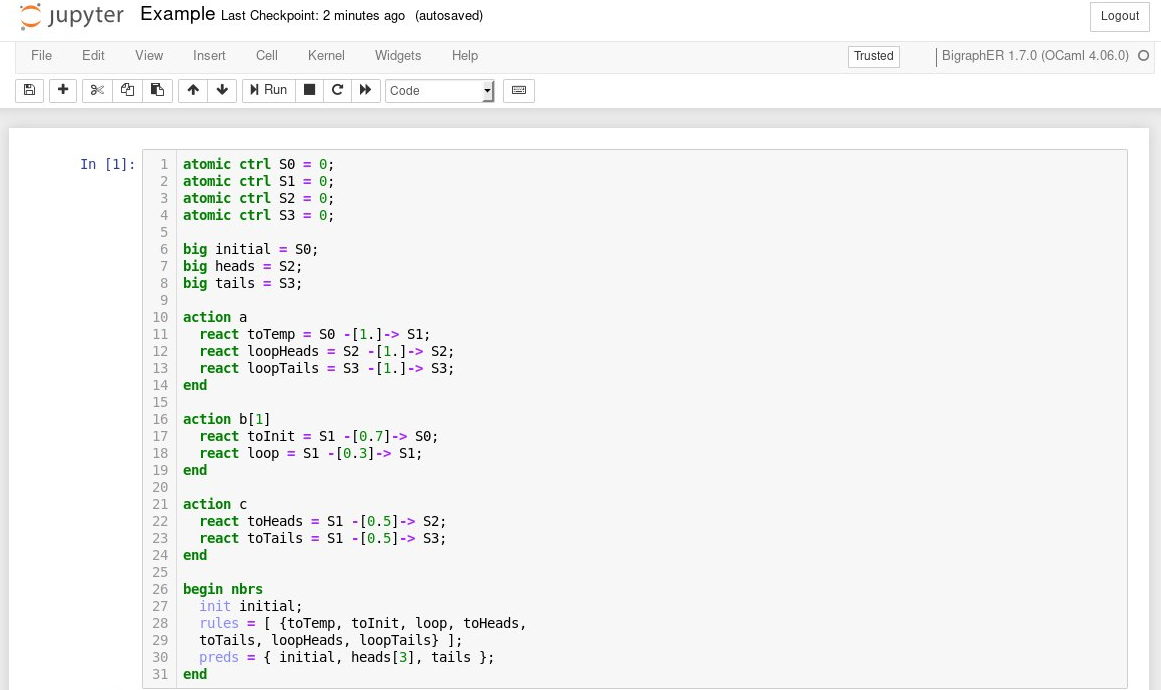
\includegraphics{images/interface.jpg}
  \caption{The BigraphER Jupyter interface with syntax highlighting.}
  \label{interface}
\end{figure}

\section{A Case Study in Autonomous Agents}

% TODO: Akin to \cite{dblp:conf/nfm/giaquintahimn18} and maybe \cite{koenig1998xavier}.

\subsection{Collecting Objects in a Grid}

% TODO: what is a link, mention that it's a hyperedge (at least one node)
% TODO: explain the syntax of the language
Our first scenario is concerned with collecting objects in a grid-like
two-dimensional world. The agent starts in the southwest corner of the map
(which we call \emph{home}), explores the environment until it collects a
specified number of objects, and returns home (while possibly collecting more
objects along the way). The model tracks which cells of the grid have been
explored, and only the unexplored cells have a constant probability $p$ of
rewarding the agent with an object. The desired number of objects can be easily
changed, and the map can be customised to make some transitions unavailable
(i.e. add walls), as long as the agent can still return home.

\lstinputlisting[caption=Controls., captionpos=b, language=Big,
label=agent1_controls, firstline=3, lastline=14]{models/agent1.big}

We begin with a list of controls in Listing \ref{agent1_controls}. On the right
hand side of each equal sign is the number of ports that each node of that
control has, while the \texttt{\textbf{atomic}} keyword specifies the nodes that
cannot contain other nodes. \texttt{Cell}s represents discrete locations. They
are linked to either \texttt{Visited} or \texttt{Unvisited} (initially, all
except one cells are unvisited). \texttt{Cell}s always contain
\texttt{Directions}, and one \texttt{Cell} contains an \texttt{Agent}. The
\texttt{Agent} may contain an \texttt{Object}. In order to represent multiple
objects, it is convenient to put the second \texttt{Object} inside the first,
and so on. \texttt{Directions} contains a subset of the four nodes,
corresponding to the four possible directions of travel: \texttt{North},
\texttt{East}, \texttt{West}, \texttt{South}. We connect neighbouring
\texttt{Cell}s by linking the \texttt{West} node of one \texttt{Cell} to the
\texttt{East} node of another (or \texttt{North} to \texttt{South}).

\lstinputlisting[caption=Predicates and the initial state., captionpos=b,
language=Big, label=agent1_code, firstline=16,
lastline=30]{models/agent1.big}

Next, we define two predicates: \texttt{home} and \texttt{goal} (see Listing
\ref{agent1_code}). The former states that the agent is home
if it is in the southwest corner of the grid,
while the latter specifies a goal of collecting one object. A larger number of
objects can be set by nesting \texttt{Object}s inside each other, e.g.,
\texttt{Agent.Object.Object}. Additionally, Listing \ref{agent1_code} defines
the initial $2 \times 2$ grid, as described previously.

\lstinputlisting[caption=The action of going north., captionpos=b,
language=Big, label=agent1_north, firstline=88,
lastline=117]{models/agent1.big}

Then, we have an action for each of the four directions, each with three
reaction rules: one for going to an already visited cell, one for visiting a
cell for the first time, and one for visiting a cell for the first time and
finding an object. We will use the rules for going north in Listing
\ref{agent1_north} as an example. When going to an already visited cell, the
\texttt{Agent} simply traverses a link between the \texttt{North} node of its
previous \texttt{Cell} and the corresponding \texttt{South} node. As this is the
only reaction rule for this situation, its probability is $1$. When going to an
unvisited node, we collect an \texttt{Object} with probability $p$, or make the
transition without getting an \texttt{Object} with probability $1-p$.
Regardless, the \texttt{Cell} changes its link from \texttt{Unvisited} to
\texttt{Visited}.

\lstinputlisting[caption=Reaction rule to stay home if a required number of
objects is acquired., captionpos=b, language=Big, label=agent1_home,
firstline=186, lastline=189]{models/agent1.big}

Lastly, we have three actions for when the agent acquires the specified number
of objects: two for going home west or south (since these are the two directions
necessary and sufficient to reach home), and one for staying home. The two
actions for going home have two reaction rules each, depending on whether the
destination cell is visited or not. They are just like the rules in Listing
\ref{agent1_north}, except every mention of \texttt{Agent} is replaced with
\texttt{goal}. The rule to stay home simply says that if the agent has achieved
the goal, and is home (characterised by a \texttt{Cell} with only two
directions: \texttt{North} and \texttt{East}), then nothing should change (see
Listing \ref{agent1_home}). To make the agent start heading home as soon as
enough objects are collected, all five reaction rules related to going and
staying home are in a higher priority class.

\subsection{Layers of Abstraction}

% TODO: Must mention: \cite{DBLP:conf/giscience/WaltonW12}.

Our second model explores two important concepts in modelling the topology of
space: nesting and uncertainty. Nesting is the idea that spaces can be inside
other spaces: rooms inside floors, floors inside buildings, buildings inside
streets, etc. A key characteristic of nested spaces is that there is a separate
action (or several) taking you from the outer space to the inner space or vice
versa (e.g., using a door to enter or leave a room). In the rest of the paper,
whenever we discuss one space inside another, we will refer to the inner space
as the \emph{room}.

The other concept explored in this section is uncertainty about the topology
itself, i.e., is the door open or closed? The implementation of this idea is
tied to that of rooms: the inside of a room is not defined until the outer cell
encompassing the room (i.e., the area where the door is located) is entered.
Then, the contents of the room are chosen from a finite set of possibilities
with a set probability distribution. After that, the room stays fixed. This
design decision supports the reality of missions with a reasonably short
duration: if the agent finds a locked door, it should not keep revisiting the
door hoping for it to suddenly be open.

As the ideas of collecting objects and tracking visited cells have been
explored already, they are dropped from this model to simplify the
implementation. The goal can simply be defined as moving from one location to
another. We add one extra control, \texttt{Node}. While \texttt{Cell} can be
imagined as a discrete patch of space (e.g., \SI{1}{\square\metre}),
\texttt{Node} can be thought of as a room. While we stick to two layers
(corridors and rooms) in this example, rooms can be freely nested: a room can
contain any number of rooms, each of which can contain more rooms.

\begin{figure}
  \centering
  \includegraphics{models/agent2/nesting_example/example.pdf}
  \caption{The bigraphical structure behind nesting.}
  \label{agent2_nesting}
\end{figure}

\lstinputlisting[caption={The initial map: three consecutive cells, the midmost
of which has an inner room.}, captionpos=b, language=Big, label=agent2_initial,
firstline=15, lastline=19]{models/agent2/agent.big}

\begin{figure}
  \centering
  \begin{minipage}{0.45\textwidth}
    \centering
    \includegraphics[width=\textwidth]{models/agent2/goIn_lhs.pdf}
  \end{minipage}
  $\longrightdoublearrowRHD$
  \begin{minipage}{0.45\textwidth}
    \centering
    \includegraphics[width=\textwidth]{models/agent2/goIn_rhs.pdf}
  \end{minipage}
  \caption{Left to right: the reaction rule to go inside; right to left: the
    reaction rule to go outside.}
  \label{go_in_out}
\end{figure}

In order to impement nesting, a \texttt{Cell} contains a \texttt{Node}, which
can have any number of \texttt{Cell}s of its own. Since after entering a room,
you end up in a specific place inside the room (next to the door), we also need
to link up the \texttt{Node} with one of the \texttt{Cell}s it contains (see
Fig. \ref{agent2_nesting}). Both \texttt{Cell}s and \texttt{Node}s support
having a single link for exactly this purpose. Thus, most of the \texttt{Cell}
ports are not linked to anything, which is implemented via closures (e.g.
\texttt{/x Cell\{x\}}). The initial map in Listing \ref{agent2_initial} has a
corridor of three cells, with the agent on the west-most cell, and a door to a
room in the middle cell. One moves in and out of a room via a pair of actions
with reaction rules pictured in Fig. \ref{go_in_out}.

\lstinputlisting[caption={Two ways to generate a room, leaving one door either
open or closed.}, captionpos=b, language=Big, label=agent2_room,
firstline=21, lastline=48]{models/agent2/agent.big}

\lstinputlisting[caption={The action of going north.}, captionpos=b,
language=Big, label=agent2_north, firstline=66,
lastline=75]{models/agent2/agent.big}

The room is a $2 \times 2$ grid of \texttt{Cell}s, which is generated when the
\texttt{Agent} gets to a \texttt{Cell} with an empty \texttt{Node} (represented
by \texttt{Node\{n\}.1}). In order for this to happen before any other action
can take place, the two reaction rules in Listing \ref{agent2_room} are put on a
higher priority class. With probability $p$, the generated room has each
\texttt{Cell} linked to its two neighbours; and with probability $1-p$, the top
two \texttt{Cell}s are not linked , possibly forcing the agent to choose a
different path. Finally, we have four actions, each with a single reaction rule
with probability $1$, corresponding to the four possible directions of travel.
The reaction rules are very similar to those of our previous example, see
Listing \ref{agent2_north}.

\section{Conclusion}

\bibliographystyle{splncs04}
\bibliography{bibliography}
\end{document}
